% ============================================================
%  MTH636 -- Game Theory | Lecture 26
%  Subgames and Subgame Perfect Equilibrium
% ============================================================
\documentclass[12pt, a4paper]{article}

% ============================================================
%  MTH636 -- Game Theory
%  Notes Preamble — Color-Coded, TikZ-Enhanced
% ============================================================

% --- Core packages ---
\usepackage[T1]{fontenc}
\usepackage[utf8]{inputenc}
\usepackage{lmodern}
\usepackage[margin=2.5cm, top=2.8cm, bottom=2.8cm]{geometry}
\usepackage{microtype}

% --- Math ---
\usepackage{amsmath, amssymb, amsthm, mathtools}
\usepackage{bm}        % bold math
\usepackage{cancel}    % strike-through in math

% --- Color & Boxes ---
\usepackage[dvipsnames, svgnames, x11names, table]{xcolor}
\usepackage[most]{tcolorbox}
\tcbuselibrary{breakable, skins, theorems}

% --- TikZ & Diagrams ---
\usepackage{tikz}
\usepackage{tikz-qtree}
\usetikzlibrary{arrows.meta, positioning, shapes.geometric, fit, backgrounds,
                decorations.pathreplacing, calc, matrix, trees}
\usepackage{pgfplots}
\pgfplotsset{compat=1.18}

% --- Tables ---
\usepackage{booktabs}
\usepackage{multirow}
\usepackage{array}
\usepackage{tabularx}
\usepackage{makecell}

% --- Typography & Layout ---
\usepackage{enumitem}
\usepackage{parskip}
\usepackage{fancyhdr}
\usepackage{titlesec}
\usepackage{titletoc}
\usepackage{hyperref}
\usepackage{graphicx}
\usepackage{float}
\usepackage{caption}

% --- Color Palette ---
\definecolor{defblue}{HTML}{1A5276}      % Definition header
\definecolor{defbluebg}{HTML}{D6EAF8}    % Definition background
\definecolor{thmgreen}{HTML}{1E8449}     % Theorem header
\definecolor{thmbg}{HTML}{D5F5E3}        % Theorem background
\definecolor{exorange}{HTML}{B7770D}     % Example header
\definecolor{exbg}{HTML}{FEF9E7}         % Example background
\definecolor{warnred}{HTML}{922B21}      % Warning/Key Insight header
\definecolor{warnbg}{HTML}{FADBD8}       % Warning background
\definecolor{noticegray}{HTML}{2C3E50}   % Note header
\definecolor{noticebg}{HTML}{EBF5FB}     % Note background
\definecolor{taketawayyellow}{HTML}{7D6608} % Key Takeaway header
\definecolor{takeawaybg}{HTML}{FDFEFE}   % Takeaway background
\definecolor{accentpurple}{HTML}{6C3483} % Accent / proof
\definecolor{lightgray}{HTML}{F2F3F4}    % shading

% ============================================================
%  TCOLORBOX ENVIRONMENTS
% ============================================================

% -- Definition (Blue) --
\newtcolorbox{defbox}[2][]{
  enhanced, breakable,
  colback=defbluebg, colframe=defblue, coltitle=white,
  fonttitle=\bfseries\sffamily,
  title={Definition: #2},
  attach boxed title to top left={yshift=-2mm, xshift=4mm},
  boxed title style={colback=defblue, rounded corners},
  arc=4pt, boxrule=1.2pt,
  left=6pt, right=6pt, top=8pt, bottom=6pt,
  #1
}

% -- Theorem / Proposition (Green) --
\newtcolorbox{thmbox}[2][]{
  enhanced, breakable,
  colback=thmbg, colframe=thmgreen, coltitle=white,
  fonttitle=\bfseries\sffamily,
  title={Theorem: #2},
  attach boxed title to top left={yshift=-2mm, xshift=4mm},
  boxed title style={colback=thmgreen, rounded corners},
  arc=4pt, boxrule=1.2pt,
  left=6pt, right=6pt, top=8pt, bottom=6pt,
  #1
}

% -- Proposition (Green variant) --
\newtcolorbox{propbox}[2][]{
  enhanced, breakable,
  colback=thmbg, colframe=thmgreen!70!black, coltitle=white,
  fonttitle=\bfseries\sffamily,
  title={Proposition: #2},
  attach boxed title to top left={yshift=-2mm, xshift=4mm},
  boxed title style={colback=thmgreen!70!black, rounded corners},
  arc=4pt, boxrule=1.2pt,
  left=6pt, right=6pt, top=8pt, bottom=6pt,
  #1
}

% -- Example (Orange/Yellow) --
\newtcolorbox{exbox}[2][]{
  enhanced, breakable,
  colback=exbg, colframe=exorange, coltitle=white,
  fonttitle=\bfseries\sffamily,
  title={Example: #2},
  attach boxed title to top left={yshift=-2mm, xshift=4mm},
  boxed title style={colback=exorange, rounded corners},
  arc=4pt, boxrule=1.2pt,
  left=6pt, right=6pt, top=8pt, bottom=6pt,
  #1
}

% -- Key Insight / Warning (Red) --
\newtcolorbox{warnbox}[2][]{
  enhanced, breakable,
  colback=warnbg, colframe=warnred, coltitle=white,
  fonttitle=\bfseries\sffamily,
  title={Key Insight: #2},
  attach boxed title to top left={yshift=-2mm, xshift=4mm},
  boxed title style={colback=warnred, rounded corners},
  arc=4pt, boxrule=1.2pt,
  left=6pt, right=6pt, top=8pt, bottom=6pt,
  #1
}

% -- Note (Gray-Blue) --
\newtcolorbox{notebox}[1][]{
  enhanced, breakable,
  colback=noticebg, colframe=noticegray!60, coltitle=white,
  fonttitle=\bfseries\sffamily,
  title={Note},
  attach boxed title to top left={yshift=-2mm, xshift=4mm},
  boxed title style={colback=noticegray!60, rounded corners},
  arc=4pt, boxrule=0.8pt,
  left=6pt, right=6pt, top=8pt, bottom=6pt,
  #1
}

% -- Key Takeaway --
\newtcolorbox{takebox}[1][]{
  enhanced, breakable,
  colback=takeawaybg, colframe=taketawayyellow, coltitle=white,
  fonttitle=\bfseries\sffamily,
  title={Key Takeaway},
  attach boxed title to top left={yshift=-2mm, xshift=4mm},
  boxed title style={colback=taketawayyellow, rounded corners},
  arc=4pt, boxrule=1.2pt,
  left=6pt, right=6pt, top=8pt, bottom=6pt,
  #1
}

% -- Intuition --
\newtcolorbox{intubox}[1][]{
  enhanced, breakable,
  colback=accentpurple!8, colframe=accentpurple!60, coltitle=white,
  fonttitle=\bfseries\sffamily,
  title={Intuition},
  attach boxed title to top left={yshift=-2mm, xshift=4mm},
  boxed title style={colback=accentpurple!80, rounded corners},
  arc=4pt, boxrule=0.8pt,
  left=6pt, right=6pt, top=8pt, bottom=6pt,
  #1
}

% ============================================================
%  PAYOFF MATRIX HELPER
%  Usage: inside tabular, use \payoff{a}{b} for (a,b)
% ============================================================
\newcommand{\payoff}[2]{$(#1,\;#2)$}
\newcommand{\nash}[2]{\underline{$#1$},\underline{$#2$}}  % underline NE payoffs
\newcommand{\Nset}{\mathbb{N}}
\newcommand{\Rset}{\mathbb{R}}
\newcommand{\Sset}{\mathcal{S}}
\newcommand{\Ui}{u_i}

% ============================================================
%  SECTION FORMATTING
% ============================================================
\titleformat{\section}
  {\large\bfseries\sffamily\color{defblue}}
  {\thesection}{1em}{}[\titlerule]

\titleformat{\subsection}
  {\normalsize\bfseries\sffamily\color{thmgreen!80!black}}
  {\thesubsection}{1em}{}

\titleformat{\subsubsection}
  {\normalsize\itshape\sffamily\color{exorange!80!black}}
  {\thesubsubsection}{1em}{}

% ============================================================
%  HEADER / FOOTER
% ============================================================
\pagestyle{fancy}
\fancyhf{}
\fancyhead[L]{\sffamily\small\color{defblue} MTH636 -- Game Theory}
\fancyhead[R]{\sffamily\small\color{defblue} \leftmark}
\fancyfoot[C]{\sffamily\small\thepage}
\renewcommand{\headrulewidth}{0.4pt}

% ============================================================
%  HYPERREF SETUP
% ============================================================
\hypersetup{
  colorlinks=true,
  linkcolor=defblue,
  urlcolor=thmgreen,
  citecolor=accentpurple,
  bookmarksnumbered=true,
  pdftitle={MTH636 Game Theory Notes},
  pdfauthor={MTH636 Student Notes}
}

% ============================================================
%  MISC HELPERS
% ============================================================
\newcommand{\BR}{\text{BR}}        % Best Response
\newcommand{\NE}{\text{NE}}        % Nash Equilibrium
\newcommand{\SPNE}{\text{SPNE}}    % Subgame Perfect NE
\newcommand{\Dom}{\text{dom}}      % Dominance
\newcommand{\mixs}[1]{\sigma_{#1}} % Mixed strategy
\newcommand{\pures}[1]{s_{#1}}     % Pure strategy


% ============================================================
\begin{document}

% Title
\begin{center}
  {\LARGE\bfseries\sffamily\color{defblue} MTH636 -- Game Theory}\\[6pt]
  {\Large\sffamily Lecture 26: Subgames and Subgame Perfect Equilibrium}\\[4pt]
\end{center}
\vspace{0.5cm}
\hrule height 1.5pt
\vspace{0.3cm}

% ============================================================
\section{Subgames of an Extensive Form Game}

Recall that a general extensive form game is denoted
\[
  \Gamma = \langle N,\, V,\, E,\, n_0,\, (V_i)_{i \in N \cup \{0\}},\,
           \mathcal{H},\, \bigl(A(h)\bigr)_{h \in \bigcup_{i} H_i},\,
           (p_n)_{n \in V_0},\, (u_i)_{i \in N} \rangle.
\]

\begin{defbox}{Subgame}
  For a game
  $\Gamma = \langle N,\, V,\, E,\, n_0,\, (V_i)_{i \in N \cup \{0\}},\,
  \mathcal{H},\, (A(h))_{h \in \bigcup_{i} H_i},\, (p_n)_{n \in V_0},\,
  (u_i)_{i \in N} \rangle$,
  a \textbf{subgame} starting at a node $y \in V$ is itself a game
  \[
    \Gamma_y = \langle N,\, V_y,\, E_y,\, y,\, (V_i)^y_{i \in N \cup \{0\}},\,
               \mathcal{H}^y,\, \bigl(A(h)\bigr)^y_{h \in \bigcup_{i} H_i},\,
               (p_n)_{n \in V_{0}^{y}},\, (u_i)_{i \in N} \rangle,
  \]
  where $V_y$ is the set of all nodes reachable from $y$, $E_y$ is the
  restriction of edges to $V_y$, and every information set $h$ must
  either be \textbf{entirely contained} in $V_y$ or entirely in
  $V \setminus V_y$.
\end{defbox}

The condition on information sets is crucial: a subgame may only begin at
a node $y$ if no information set is ``split'' by $y$ -- that is, no
information set contains both a node inside $V_y$ and a node outside $V_y$.

\subsection{Illustrative Examples of Subgames}

\subsubsection*{Example 1 -- Battle of the Sexes (extensive form)}

Consider the sequential Battle of the Sexes game. The Man (player M)
moves first at the root $n_0$ and can choose $F$ (Football) or $D$ (Dance).
The Woman (player W) then moves at the resulting node.

\begin{center}
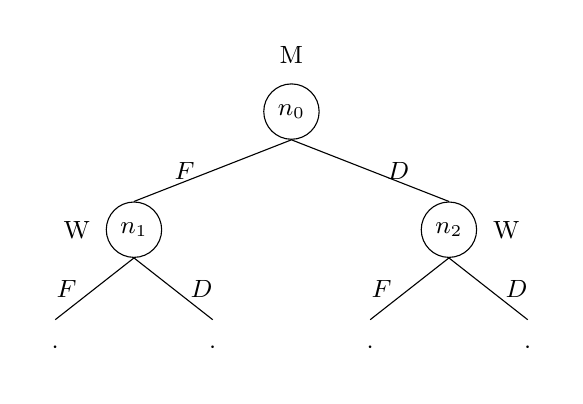
\begin{tikzpicture}[
    level 1/.style={sibling distance=4cm},
    level 2/.style={sibling distance=2cm},
    every node/.style={draw, circle, minimum size=0.7cm, font=\small}
  ]
  \node[label=above:{M}] (n0) {$n_0$}
    child { node[label=left:{W}] {$n_1$}
              child { node[draw=none] {$\cdot$} edge from parent node[left,draw=none] {$F$} }
              child { node[draw=none] {$\cdot$} edge from parent node[right,draw=none] {$D$} }
            edge from parent node[left,draw=none] {$F$} }
    child { node[label=right:{W}] {$n_2$}
              child { node[draw=none] {$\cdot$} edge from parent node[left,draw=none] {$F$} }
              child { node[draw=none] {$\cdot$} edge from parent node[right,draw=none] {$D$} }
            edge from parent node[right,draw=none] {$D$} };
\end{tikzpicture}
\end{center}

Here the information set of the Woman (player W) is $\{n_1, n_2\}$, shown
with a dashed arc connecting the two nodes. Because both $n_1$ and $n_2$
belong to the \emph{same} information set, neither $n_1$ alone nor $n_2$
alone can serve as the root of a subgame -- the information set would be
split. The \emph{only} proper subgame is the entire game itself (i.e.\ the
game is its own unique subgame).

\subsubsection*{Example 2 -- Three-player game with information sets}

Consider a game with three players I, II, III whose tree has nodes
$n_0, n_1, \ldots, n_6$.
\begin{itemize}
  \item Player I moves at $n_0$ (actions $A$ and $B$).
  \item Player II has an information set $\{n_1, n_2\}$ and moves with
        actions $\ell$ and $r$ (from $n_1$) and $L$, $R$ (from $n_2$).
  \item Player III has an information set $\{n_3, n_4, n_5, n_6\}$ and
        takes actions $a$, $b$ at each node.
\end{itemize}

Because player III's information set $\{n_3,n_4,n_5,n_6\}$ spans nodes
reached via \emph{both} branches of player I's move, no subgame can be
started at any node $n_3, \ldots, n_6$ individually. The entire game is
therefore its own only subgame.

% ============================================================
\section{Subgame Perfect Equilibrium (SPE)}

\begin{defbox}{Subgame Perfect Equilibrium (SPE)}
  A strategy profile $\sigma$ is a \textbf{Subgame Perfect Equilibrium
  (SPE)} if it is a Nash Equilibrium in \emph{all} subgames of the game.
\end{defbox}

SPE refines Nash Equilibrium by eliminating non-credible threats: a player
cannot credibly threaten to take a suboptimal action in a subgame that would
never be reached in equilibrium, because the SPE requirement forces rational
play even in off-path subgames.

% ============================================================
\section{Examples of Finding SPE}

\subsection*{Example A}

Consider a two-player sequential game with the following structure. Player I
moves first at $n_0$ choosing $L$ or $R$. After $L$ the game reaches a
subgame at $n_2$ where player II chooses $\ell$ or $r$; the payoff from $L$
alone is $(1, -1)$. After $R$ the game reaches a subgame at $n_3$ where
player II again chooses $\ell$ or $r$.

\medskip
\noindent The terminal payoffs are:
\begin{center}
  \begin{tabular}{c|cc}
             & $\ell$    & $r$     \\
    \hline
    $L$      & $(1,-1)$  & $(-1,1)$\\
    $R$      & $(-1,1)$  & $(1,-2)$\\
  \end{tabular}
\end{center}

\noindent\textbf{Nash Equilibria found:} $(L, \ell)$ and $(-1, 1)$ -- two
NE exist.

\noindent\textbf{SPE:} $(L, \ell)$ -- only one SPE.

Observe the game tree with player I at $n_0$ branching into $L$ (to $n_2$,
player II) and $R$ (to $n_3$, player II), where player II's information set
$\{n_2, n_3\}$ is circled. The four terminal payoffs are
$(1,-1),(-1,1),(-1,1),(1,-2)$ from left to right.

\begin{notebox}
  There are two Nash Equilibria $(L, \ell)$ and $(-1, 1)$, but \emph{only
  one} SPE: $(L, \ell)$.
\end{notebox}

\subsection*{Example B -- Two-stage sequential game}

Player I moves at $n_0$: actions $A$ or $B$.
\begin{itemize}
  \item If $A$: payoff $(1, 2)$ immediately.
  \item If $B$: play reaches player II at node $u_1$, who chooses $C$ or
        $D$, giving payoffs $(0,0)$ or $(2,1)$ respectively.
\end{itemize}

\medskip
\noindent\textbf{Game tree:}
\begin{center}
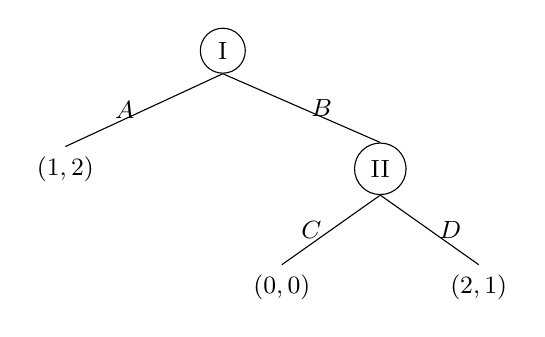
\begin{tikzpicture}[
    level 1/.style={sibling distance=4cm},
    level 2/.style={sibling distance=2.5cm},
    every node/.style={font=\small}
  ]
  \node[draw,circle] (I) {I}
    child { node[draw=none] {$(1,2)$} edge from parent node[left,draw=none] {$A$} }
    child { node[draw,circle] {II}
              child { node[draw=none] {$(0,0)$} edge from parent node[left,draw=none] {$C$} }
              child { node[draw=none] {$(2,1)$} edge from parent node[right,draw=none] {$D$} }
            edge from parent node[right,draw=none] {$B$} };
\end{tikzpicture}
\end{center}

\noindent The normal form matrix (Player I rows, Player II columns):
\begin{center}
  \begin{tabular}{c|cc}
           & $C$    & $D$    \\
    \hline
    $A$    & \payoff{1}{2} & \payoff{1}{2} \\
    $B$    & \payoff{0}{0} & \payoff{2}{1} \\
  \end{tabular}
\end{center}

\noindent\textbf{Two NE:} $(A, C)$ and $(B, D)$.

\noindent\textbf{One SPE:} $(B, D)$.

The strategy $(A, C)$ is an NE: if Player I plays $A$, Player II's choice
is irrelevant (payoff is $(1,2)$ regardless). However, if the game ever
reached Player II's node, Player II would prefer $D$ (payoff 1 to II) over
$C$ (payoff 0). The threat of $C$ is non-credible. The SPE is therefore
$(B, D)$.

\subsection*{Example C -- Mixed strategy NE and SPE}

Consider the same game structure as Example B but now allowing mixed
strategies. The NE of the game are:
\[
  (A,\, \alpha[C] + (1-\alpha)[D]), \quad \alpha \geq \tfrac{1}{2}
\]
and $(B, D)$.

The SPE are those NE that also constitute an NE in the subgame rooted at
player II's node. In the subgame at $n_1$:
\begin{center}
  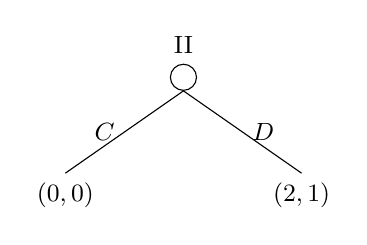
\begin{tikzpicture}[
      level 1/.style={sibling distance=3cm},
      every node/.style={font=\small}
    ]
    \node[draw,circle,label=above:{II}] {}
      child { node[draw=none] {$(0,0)$} edge from parent node[left,draw=none] {$C$} }
      child { node[draw=none] {$(2,1)$} edge from parent node[right,draw=none] {$D$} };
  \end{tikzpicture}
\end{center}

In the subgame $\Gamma_{n_1}$, the strategy $\alpha[C] + (1-\alpha)[D]$ is
\emph{not} an NE if $\alpha > 0$: Player II strictly prefers $D$ (payoff 1)
over $C$ (payoff 0). Therefore only $D$ is an NE of the subgame.

\begin{itemize}
  \item The mixed strategy $(A,\, \alpha[C]+(1-\alpha)[D])$ with $1 > \alpha
        \geq \tfrac{1}{2}$: \textbf{SPE} (Player I plays $A$, so subgame is
        off-path; but Player II must play $D$ in the subgame -- contradiction
        with $\alpha>0$). \emph{Not} an SPE for $\alpha > 0$.
  \item $(B, D)$: \textbf{SPE}.
\end{itemize}

\begin{notebox}
  $(\alpha[C],\,(1-\alpha)[D])$ is not an NE of the subgame at $n_1$ for any
  $\alpha > 0$. The only NE of that subgame is $D$. Therefore the unique SPE
  is $(B, D)$.
\end{notebox}

\subsection*{Example D -- Larger sequential game}

\noindent Player I at $n_0$ chooses $A$ or $B$.
\begin{itemize}
  \item $A \to$ payoff $(1,2)$.
  \item $B \to$ Player II at node with children $n_3$ (from $C$) and
        $n_5$ (from $D$).
        \begin{itemize}
          \item $C \to$ payoff $(0,0)$.
          \item $D \to$ payoff $(1,1)$.
        \end{itemize}
\end{itemize}

\noindent Normal form:
\begin{center}
  \begin{tabular}{c|cc}
           & $C$    & $D$    \\
    \hline
    $A$    & \payoff{1}{2} & \payoff{1}{2} \\
    $B$    & \payoff{0}{0} & \payoff{1}{1} \\
  \end{tabular}
\end{center}

\noindent NE of the game: $(A,C)$ (not SPE), $(A,D)$ (SPE), and
$\left(\tfrac{1}{2}[A]+\tfrac{1}{2}[B],\, D\right)$ (SPE).

\noindent $(B, D)$ is also an SPE.

\begin{takebox}
  The SPE concept eliminates Nash Equilibria that rely on non-credible
  threats. Whenever a player's strategy prescribes an action in a subgame
  that is irrational for that player (given the subgame), that NE is
  \emph{not} an SPE.
\end{takebox}

\end{document}
